\documentclass{article}
\usepackage{icmcsmc2014}
\usepackage{times}
\usepackage{ifpdf}
\usepackage[english]{babel}
%\usepackage{cite}
\usepackage{fancyvrb}
%%%%%%%%%%%%%%%%%%%%%%%% Some useful packages %%%%%%%%%%%%%%%%%%%%%%%%%%%%%%%
%%%%%%%%%%%%%%%%%%%%%%%% See related documentation %%%%%%%%%%%%%%%%%%%%%%%%%%
%\usepackage{amsmath} % popular packages from Am. Math. Soc. Please use the 
%\usepackage{amssymb} % related math environments (split, subequation, cases,
%\usepackage{amsfonts}% multline, etc.)
%\usepackage{bm}      % Bold Math package, defines the command \bf{}
%\usepackage{paralist}% extended list environments
%%subfig.sty is the modern replacement for subfigure.sty. However, subfig.sty 
%%requires and automatically loads caption.sty which overrides class handling 
%%of captions. To prevent this problem, preload caption.sty with caption=false 
%\usepackage[caption=false]{caption}
%\usepackage[font=footnotesize]{subfig}


%user defined variables
\def\papertitle{Advances in Modality}
\def\firstauthor{First author}
\def\secondauthor{Second author}
\def\thirdauthor{Third author}


% authors so far:
% AdC, Till, Jeff

% adds the automatic
% Saves a lot of ouptut space in PDF... after conversion with the distiller
% Delete if you cannot get PS fonts working on your system.

% pdf-tex settings: detect automatically if run by latex or pdflatex
\newif\ifpdf
\ifx\pdfoutput\relax
\else
   \ifcase\pdfoutput
      \pdffalse
   \else
      \pdftrue
\fi

\ifpdf % compiling with pdflatex
  \usepackage[pdftex,
    pdftitle={\papertitle},
    pdfauthor={\firstauthor, \secondauthor, \thirdauthor},
    bookmarksnumbered, % use section numbers with bookmarks
    pdfstartview=XYZ % start with zoom=100% instead of full screen; 
                     % especially useful if working with a big screen :-)
   ]{hyperref}
  %\pdfcompresslevel=9

  \usepackage[pdftex]{graphicx}
  % declare the path(s) where your graphic files are and their extensions so 
  %you won't have to specify these with every instance of \includegraphics
  \graphicspath{{./figures/}}
  \DeclareGraphicsExtensions{.pdf,.jpeg,.png}

  \usepackage[figure,table]{hypcap}
\fi

%setup the hyperref package - make the links black without a surrounding frame
\hypersetup{
    colorlinks,%
    citecolor=black,%
    filecolor=black,%
    linkcolor=black,%
    urlcolor=black
}


% Title.
% ------
\title{\papertitle}

% Authors
% Please note that submissions are NOT anonymous, therefore 
% authors' names have to be VISIBLE in your manuscript. 
%
% Single address
% To use with only one author or several with the same address
% ---------------
%\oneauthor
%   {\firstauthor} {Affiliation1 \\ %
%     {\tt \href{mailto:author1@smcnetwork.org}{author1@smcnetwork.org}}}

%Two addresses
%--------------
% \twoauthors
%   {\firstauthor} {Affiliation1 \\ %
%     {\tt \href{mailto:author1@smcnetwork.org}{author1@smcnetwork.org}}}
%   {\secondauthor} {Affiliation2 \\ %
%     {\tt \href{mailto:author2@smcnetwork.org}{author2@smcnetwork.org}}}

% Three addresses
% --------------
 \threeauthors
   {\firstauthor} {Affiliation1 \\ %
     {\tt \href{mailto:author1@smcnetwork.org}{author1@smcnetwork.org}}}
   {\secondauthor} {Affiliation2 \\ %
     {\tt \href{mailto:author2@smcnetwork.org}{author2@smcnetwork.org}}}
   {\thirdauthor} { Affiliation3 \\ %
     {\tt \href{mailto:author3@smcnetwork.org}{author3@smcnetwork.org}}}


% ***************************************** the document starts here ***************
\begin{document}
%
\capstartfalse
\maketitle
\capstarttrue
%
\begin{abstract}
\end{abstract}

\begin{figure}[h]
	\centering
		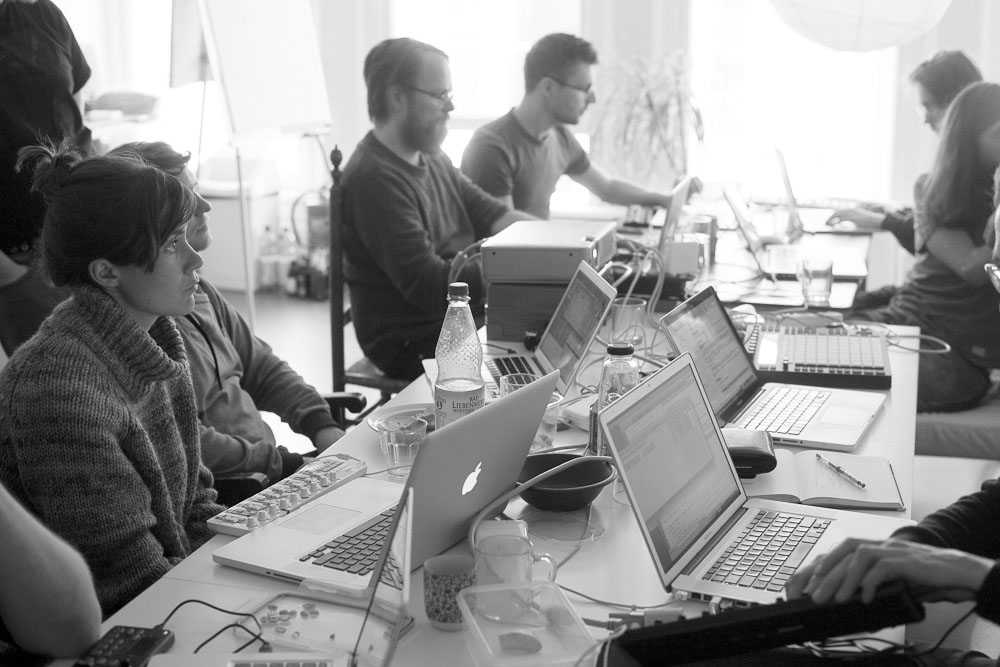
\includegraphics[width=.9\columnwidth]{../media/20140331-IMG_5976.jpg}
	\caption{Meeting 2014 in Amsterdam}
	\label{fig:media_20140331-IMG_5976}
\end{figure}

\section{Overview of the modality concept and its aims}
\label{sec:overview_of_modality_concept_and_aims}

Modality is a project dedicated to modal interaction with synthesis processes for physical control in performance. Its primary product is the Modality Toolkit, a library to facilitate straightforward access to hardware controllers in the SuperCollider programming language. It is designed and developed by the ModalityTeam, a group of people that see themselves as both users and developers both of and for SuperCollider.

The idea behind the Modality Toolkit is to simplify the creation of individual electronic instruments using controllers of various kinds. 
To this end, a common code interface, MKtl, is used for connecting controllers from various sources and protocols. 
Currently HID and MIDI are supported with OSC, GUI-based interfaces can be created on the fly from interface descriptions.


\section{Scope of Modality}
\label{sec:scope_of_modality_tech_info_where_what}

\emph{Tells about the scope of the modality group, how it was established and how the meetings work. Should especially include a description of the combination of developer meeting, public workshop and concert.}

The name Modality arose from the idea to scaffold the creation of modal interfaces, i.e., to create interfaces where e.g. one physical controller can be used for different purposes or it is possible to switch its functionality, even at runtime. It is our belief that integration of such on-the-fly remapping features helps to create instruments that are flexible, powerful, and interesting to play. The strength of such a modal interface is that it allows for fast changes and more opportunity for sonic discovery as can be necessary when, for example, improvising with musicians playing acoustic instruments. 


\subsection{Unifications of interface implementations}
\label{sub:unifications_of_interface_implementations}

With MKtl, it is possible to assign functionality to controller elements.
Each MKtl object has elements such as sliders or knobs. It is possible to assign an action to such an element that is evauated every time, the value of that element gets updated. Below, there are two examples using popular MIDI controller.

\begin{Verbatim}
k = MKtl('nnkn20');
\end{Verbatim}



\begin{itemize}
	\item Modality toolkit + Various Mixed Things + closely related
	\item more related libs - FP/FRP, wslib, JITLibExtensions, 
		all of Marijes device related quarks, etc 
\end{itemize}

\begin{figure}[h]
	\centering
		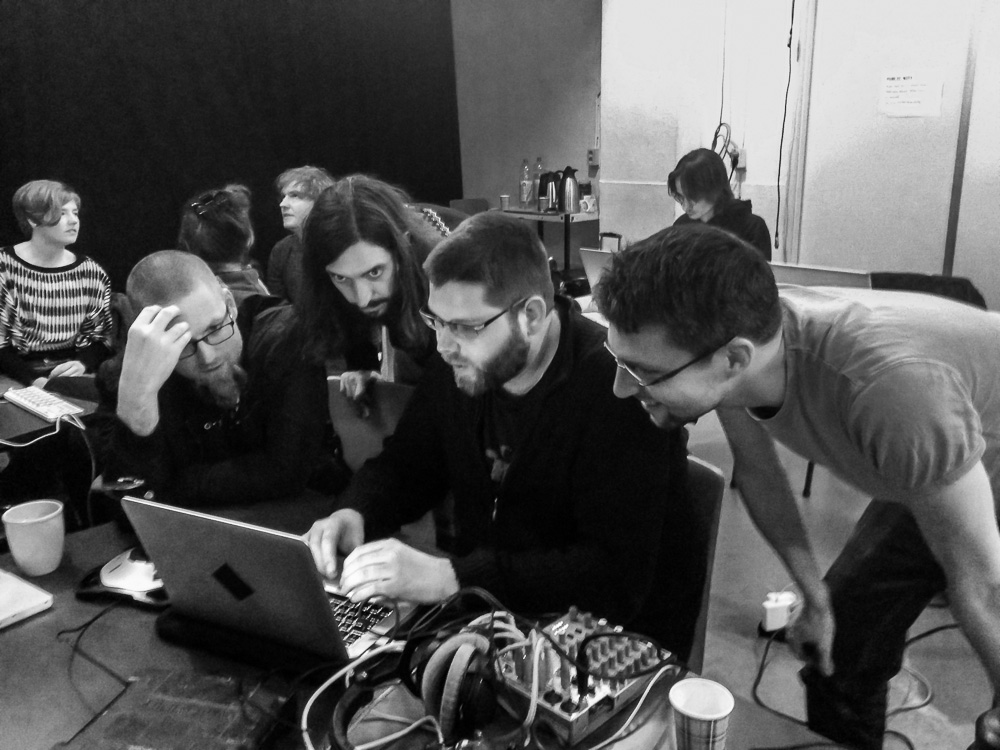
\includegraphics[width=.9\columnwidth]{../media/20140403-IMG_1667.jpg}
	\caption{Public workshop and open Lab at STEIM}
	\label{fig:media_20140331-IMG_5976}
\end{figure}


\section{Descriptions files}
\label{sec:descriptions_files}

A controller is always bound to one protocol. 
If there is a device that communicates on multiple protocols (e.g. ICON i-controls), it has to be merged later in the processing chain. 
A control element is a part of a controller that generates a one-dimensional stream of events, accepts a one-dimensional stream of events or both of the above.

The functionality of MKtl relies on descriptions of the used devices. 
A description file gathers information for each control element. 
One line in the description is a combination of (a) semantic information (e.g. for searching or automated grouping) and (b) technical information that is used to get information on how the element can be accessed internally.
It is of this form:
\begin{Verbatim}
\key: (\infoKey: infoVal, \infoKey: infoVal, ...),
\end{Verbatim}
Elements can also be hierarchically grouped:
\begin{Verbatim}
\elemkey: [
	[
		\key: (\infoKey: infoVal, \infoKey: infoVal, ...),
		\key: (\infoKey: infoVal, \infoKey: infoVal, ...),
	],[
		...
	]
]
\end{Verbatim}


\section{Islands and Bridges, uniform protocols}
\label{sec:islands_and_bridges_uniform_protocols}

Uniform devices (MIDI, HID, OSC, GUI, Serial)
		with rich descriptions, hierarchical names for all elements
		FakeGUI for everything


	
	Uniform destinations:
		set messages, RelSet, SoftSet, // if Influx, influence
		
\begin{figure}[h]
	\centering
		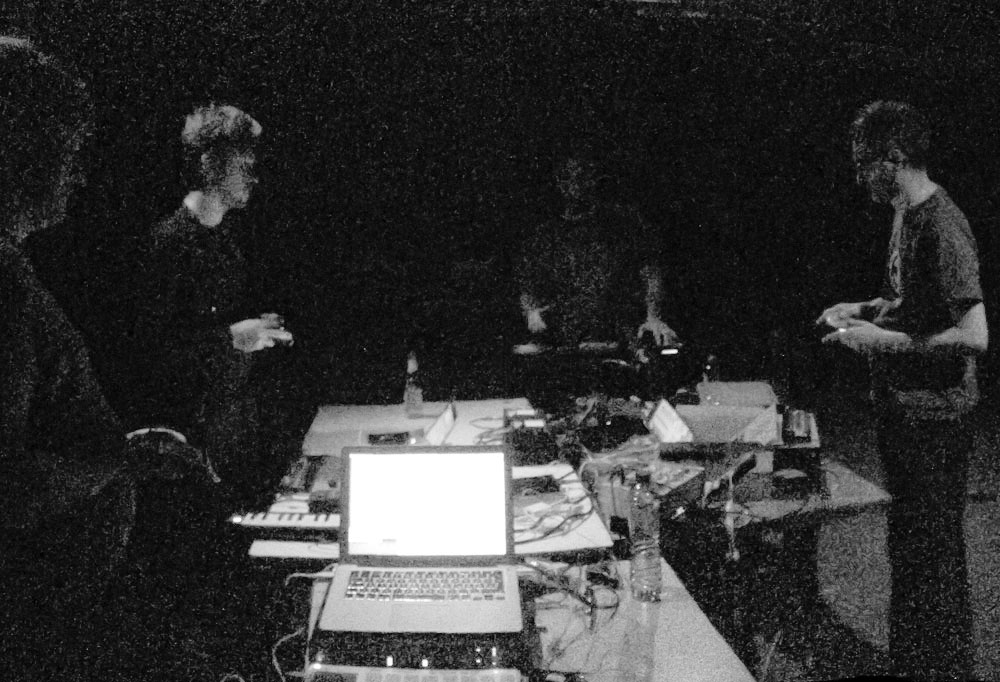
\includegraphics[width=.9\columnwidth]{../media/20140405-IMG_1691.jpg}
	\caption{Modality Concert 2014 at OT301}
	\label{fig:media_20140405-IMG_1691}
\end{figure}

\section{Methods}
\label{sec:methods}

Transformer islands: 
		FRP, Influx, others 
		- process incoming events, pass on results to destinations.

\section{Examples / Use Cases}
\label{sec:examples_use_cases}




\subsection{MPD 18}
\label{sub:mpd_18}

The MPD18 has 16 Buttons and a slider.

    [Sound Buttons] Buttons 1-3 are mapped to adsr enveloped sound sources.
        By pushing them down sound turns on; releasing: sound off.
    the Slider sets amplitude (or pitch) for the (sound)source of the currently depressed button.
    [Memory Slots] Buttons 5-16 represent 'memory' positions (initially not mapped)
        if sound is assigned (see below), sound is played when button depressed.
    [Shift Button] Button 4 is a 'shift key'. When depressed
        Sound Buttons don't trigger any sound but select the active slot. This can be followed by
        depressing a Memory Slot button, which assigns the selected sound to that pad.
        if you release the shift key before assignment, nothing happens.
        assigning a copy to an already assigned memory slot replaces existing
        mute copy +[Sound Button then Shift button]
        Sound Button triggers sound
        depress Memory Slot button, assigning the sound to the pad, with sound

\subsection{Switching actions}
\label{sub:switching_actions}




\section{Conclusions}
\label{sec:conclusions}


Modality - it's THE THING, yo!


\begin{acknowledgments}
The Modality team is (in alphabetical order):
    Marije Baalman,
	Tim Blechmann,
    Till Bovermann,
    Alberto de Campo,
    Jeff Carey,
    Bjoernar Habbestad,
	Dominik Hildebrand Marques Lopes,
	Amelie Hinrichsen,
    Robert van Heumen,
    Hannes Hoelzl,
    Miguel Negrao, and
    Wouter Snoei.
Associated organisations are (in alphabetical order):
BEK,
the project \emph{Design, Development and Dissemination of New Musical Instruments} of UdK Berlin/TU Berlin, supported by the Einstein Foundation,
nescivi, and
STEIM.

\end{acknowledgments} 

%%%%%%%%%%%%%%%%%%%%%%%%%%%%%%%%%%%%%%%%%%%%%%%%%%%%%%%%%%%%%%%%%%%%%%%%%%%%%
%bibliography here
\bibliography{smacsmc2014template}

\end{document}
